%Template for PLoS
% Version 1.0 January 2009
%
% To compile to pdf, run:
% latex plos.template
% bibtex plos.template
% latex plos.template
% latex plos.template
% dvipdf plos.template
\documentclass[12pt]{article}

% amsmath package, useful for mathematical formulas
\usepackage[utf8]{inputenc}
\usepackage[T1]{fontenc}
\usepackage{amsmath}
\usepackage[mathlines,displaymath]{lineno}
\usepackage{mathtools}
% amssymb package, useful for mathematical symbols
\usepackage{amssymb}
\usepackage{natbib}
\usepackage[usenames,dvipsnames,table]{xcolor}
% graphicx package, useful for including eps and pdf graphics
% include graphics with the command \includegraphics
\usepackage{graphicx}
\usepackage{times}
\usepackage{tikz}
\usepackage{amsmath}
\usepackage{verbatim}
\usepackage{animate}
\usepackage{float}
\usepackage{boxedminipage}
\usepackage{color}
%\usepackage[portuguese]{babel}
\newcommand{\carlos}[1]{\textcolor{Red}{#1}}
\newcommand{\GM}[1]{\textcolor{Blue}{#1}}
\newcommand{\JK}[1]{\textcolor{Green}{#1}}

\usetikzlibrary{arrows,shapes}

% cite package, to clean up citations in the main text. Do not remove.
%\usepackage{cite}

\usepackage{color} 

% package multirow for advanced formatting if tables
\usepackage{multirow}

% Use doublespacing - comment out for single spacing
%\usepackage{setspace} 
%\doublespacing


% Text layout
\topmargin 0.0cm
\oddsidemargin 0.5cm
\evensidemargin 0.5cm
\textwidth 16cm 
\textheight 20cm

% Bold the 'Figure #' in the caption and separate it with a period
% Captions will be left justified
\usepackage[labelfont=bf,labelsep=period,justification=raggedright]{caption}

% Remove brackets from numbering in List of References
\makeatletter
\renewcommand{\@biblabel}[1]{\quad#1.}
\makeatother

% Leave date blank
\date{}
%\doublespacing

\pagestyle{myheadings}

\begin{document}

\begin{flushleft}
{\Large
\textbf{Metacommunities in dynamic landscapes}
}
%% Insert Author names, affiliations and corresponding author email.
\\
\vspace{1.0cm} Charles N. de Santana$^{1,2,4,\ast}$, Jan
Klecka$^{1,3,\ast}$, Gian M. Palamara$^{4}$, Carlos J. Meli\'an$^{1}$
\\
\vspace{1.0cm} \bf{1} Department of Fish Ecology and Evolution, EAWAG,
Swiss Federal Institute of Aquatic Science and Technology, Switzerland
\\
\bf{2} Programa de Pos-Graduaç\~{a}o em Ciencias da Terra e do Ambiente,
Universidade Estadual de Feira de Santana, Bahia, Brasil
\\
\bf{3} Laboratory of Theoretical Ecology, Institute of Entomology,
Biology Centre of the Czech Academy of Sciences, \v{C}esk\'{e}
Bud\v{e}jovice, Czech Republic\\
\bf{4} Institute of Evolutionary Biology and Environmental Studies, University of Zurich, Switzerland\\
  \vspace{0.5 in}
  
  Keywords: patch dynamics, connectivity dynamics, seasonality, climate fluctuations\\
  population dynamics, individual based model, random geometric networks,\\
  regional species richness, static landscapes, dynamic landscapes.\\
  Type of Article: Article\\
  Number of figures: 7 (5 in color); Number of tables: 2\\
$\ast$ Shared first authors\\
$\ast$ Corresponding author: charles.desantana@eawag.ch\\
\end{flushleft}

\newpage
% Please keep the abstract between 250 and 300 words
\section*{Abstract}
Predictions from theory and experiments have shown that high landscape connectivity promotes higher species richness than low connectivity. However, this pattern is not general because examples demonstrating high diversity in low connected landscapes also exist. Landscape connectivity depends on factors which show intraday and daily to seasonal or larger time scale fluctuations but their role to understand the effect of the fluctuations of landscape connectivity on species richness is lacking in metacommunity theory. Here, we connect the many factors that drive landscape connectivity by varying the amplitude and frequency of the change in the dispersal radius to show that the fluctuations of landscape connectivity play a key role in predicting species richness. Our results show that the mean species richness (i.e., mean $\gamma-$species richness) decays as the landscape becomes more and more fragmented in several isolated components both in static and dynamic landscapes. However, the variance of $\gamma-$species richness peaks with an intermediate number of isolated components in dynamic landscapes suggesting high $\gamma-$species richness can also occur in dynamic landscapes with a large number of isolated components. Our results also show a dispersal radius threshold below which species richness drops dramatically in static landscapes. Such a threshold disappears for dynamic landscapes for a broad range of amplitude and frequency values of dispersal radius determining landscape connectivity. We conclude that merging amplitude and frequency of fluctuations of landscape connectivity together with patch dynamics into metacommunity theory can provide new testable predictions about species diversity in fast-changing landscapes.

\newpage
\section*{Introduction}

Metacommunity theory provides a number of insights into the role of dispersal for species coexistence in landscapes composed of units of suitable and unsuitable habitats. Theoretical and empirical studies have shown that different spatial processes can drive persistence and species richness (\cite{Holyoaketal2005}). Empirical studies have largely focused on dispersal rates with only recent emphasis on patterns of landscape connectivity (\cite{kneitel2004, cadotte2006}). Most results have shown that increasing connectivity tends to increase persistence and richness (\cite{ellneretal2001, foxetal2011}), but examples of decreasing richness with increasing connectivity are also known (\cite{daviesetal2009, altermattetal2011}). Theoretical models predict that habitat loss and fragmentation may reach a threshold beyond which there is a rapid avalanche of species extinctions (\cite{fahrig2002,ovaskainenhanski2003,rybickihanski2013}). These predictions gained empirical support from studies of deforestation where a transition from a continuous forest to more isolated and smaller fragments of the original habitat occurs and is accompanied by significant species loss (\cite{LauranceEtAl1997, MetzgerEtAl2009}). In this case, habitat destruction increases the distance between remaining patches which decreases landscape connectivity and disrupts dispersal of organisms. Apart from such directional changes, fluctuations in landscape availability (random or seasonal) are also common in nature (\cite{Sprugel1991, RuizEtAl2014}) but their consequences for species richness received less attention, with the exception of disturbances (\cite{Sousa1984, SuppErnest2014}). Whether landscape connectivity increases or decreases persistence and regional species richness, dispersal abilities of organisms, which define habitat connectivity, are affected by the fluctuations in the environment and various habitat characteristics. Many of these factors fluctuate with different frequencies, with some showing high intraday variation while others fluctuate daily, seasonally or at larger time scales (figure 1) (\cite{StensethEtAl2002}). The spatial extent of these processes can be described using the amplitude and frequency of the fluctuations.

Landscape dynamics encompasses two major processes i.e., patch dynamics and variation in landscape connectivity. Patch dynamics is defined as changes of the number and position of patches, changes of patch habitat characteristics, size and suitability. Fluctuations in landscape connectivity is defined as changes in the property of the matrix organisms have to cross to disperse from one patch or habitat to another (table 1). Variation in patch dynamics and landscape connectivity at all spatial and temporal scales may affect species richness and community structure. In some cases, the temporal and spatial scales are correlated; i.e. large-scale changes occur infrequently or slowly over a long time. Classic examples include fast gap dynamics in grasslands caused by animals (\cite{WhickerDetling1988, HobbsMooney1991, MiltonEtAl1997}) and slower forest dynamics caused by individual tree-falls (\cite{Goldblum1997}) and larger-scale fires (\cite{VanWagnerEtAl2006, WhelanEtAl2013}) (figure 1). At large temporal scales, transitions between habitat types at the continental scale occur during glacial-interglacial cycles (\cite{WerneckEtAl2011}). However, there are also examples of large-scale landscape dynamics over short time scales, such as daily tides and seasonal changes of sea ice extent, which demonstrate that coupling of temporal and spatial scales is not a general phenomenon (figure 1). These types of landscape dynamics may have profound implications for population dynamics of many organisms. These fluctuations may alter the impact of climate change velocity on threatened populations (\cite{loarieetal2009}), affect population divergence and speciation (\cite{aguileetal2011}), and drive changes of the latitudinal biodiversity gradient over time (\cite{mannionetal2014}).

Patch dynamics, i.e. the process of destruction of patches and appearance of new ones has been addressed by numerous theoretical studies of metapopulations (\cite{Hanski1999,Cornell&Ovaskainen2008,DrechslerJohst2010}). For example \cite{Hanski1999} derived formulas for predicting patch occupancy of a single population in landscapes with this type of patch dynamics. The mean species lifetime in a network of dynamical patches can also be estimated (\cite{DrechslerJohst2010}). Recent studies have shown that the rate of patch turnover is critical for metapopulation persistence. For example, \citet{reigadaetal2015} showed that increasing the rate of patch dynamics, i.e. patches are very ephemeral, decreases metapopulation persitence when dispersal is continuous, while persistence is facilitated by pulsed dispersal. The links connecting different patches can also vary in time. For example, the connectivity of habitat patches in the polar regions fluctuates seasonally according to the extend of sea ice (figure 1 and animations SI-A1 and SI-A2). Wetlands are a good example where seasonal changes in precipitations drive strong seasonal fluctuations of landscape connectivity as individual water bodies connect during heavy rains and floods and become isolated during the dry season (\cite{RoshierEtAl2008, RuizEtAl2014}). Connectivity dynamics can therefore be critical in determining landscape structure. However, connectivity dynamics has received less attention in metacommunity and metapopulation ecology (\cite{Holyoaketal2005,JohstEtAl2011}). This is likely because more focus on simple analytically tractable models, but its complementarity to more complex stochastic models can be extremely useful to increase robustness in model inference and to build synthesis by merging concepts from many disciplines \citep{EvansEtAl2013}}. The concept of connectivity dynamics has been more commonly used in disease ecology (\cite{Dushoffetal2004,Keeling&Eames2005,Ross2010}). For example, sinusoidal forcing of the transmission rate can more accurately describe fluctuations of incidence in the host as observed in the dynamics of the host–influenza system (\cite{Dushoffetal2004}).

Despite the scarcity of theoretical predictions, there is a lot of empirical evidence that connectivity dynamics may play an important role for dynamics of metapopulations in heterogeneous landscapes. Most of the empirical evidence comes from studies which focused on single-species metapopulation persistence. It is important to realize that habitat connectivity is driven by the characteristics of the landscape matrix separating habitat patches as perceived by the organisms (\cite{EycottEtAl2012}). For example, dispersal of amphibians between ponds is strongly affected by the terrestrial habitat separating the ponds (\cite{VanBuskirk2012, ClineHunter2014}) and by weather (e.g., moisture) (\cite{RittenhouseEtAl2009}). Similarly, dispersal of butterflies also depends on the matrix environment (\cite{KueflerEtAl2010}) and dispersal kernels fluctuate in time (\cite{SchtickzelleEtAl2012}). In fish, interconnections between rivers forming during periods of heavy rain can connect otherwise disconnected habitats and allow for dispersal and gene flow (\cite{BoizardEtAl2009}). Despite these empirical observations, mechanisms to study fluctuations of landscape connectivity has been rarely included in metacommunity studies. Here, we study the effect of amplitude and frequency of change of dispersal radius of organisms, as a determinant of landscape connectivity, on regional species richness. Figure 1 illustrates the range of temporal and spatial scales that can be studied using the amplitude and frequency of change of organismal dispersal radius as determinants of changes in landscape connectivity. We first aim to identify gaps in our knowledge of the patch and connectivity dynamics as the mechanisms driving species diversity in metacommunities (figure 2, table 1 for a glossary of main concepts). We then describe in detail our approach by comparing landscapes with no connectivity change (i.e., static landscapes) with the role of amplitude and frequency of fluctuations of dispersal radius for landscape connectivity and regional species richness (i.e., dynamic landscapes, table 2 and figures 3-4). Any fluctuating signal with a given amplitude and frequency can be described using its mean and variance. For example, a perfectly sinusoidal signal, measured along an integer number of periods, will have a variance proportional to the amplitude of the signal and a mean given by one half of the difference between the maximum and the minimum (figure 3). This scenario describes a correlation between the mean dispersal radius for organisms to move between patches and the variance of this radius and it resembles a temporal and spatial correlation in some environmental factors (figure 4). The second scenario explores large-landscape dynamics over short time scales, such as daily tides and seasonal changes of sea ice extent, which mean decoupled temporal and spatial scales. Thus it assumes that the mean and the variance of dispersal radius are independent of each other (\cite{Violletal2012}) (figure 3). We compare predictions from these two scenarios with static landscapes where connectivity is constant (figures 5-7). Finally, we propose a road-map for incorporating landscape dynamics more realistically into metacommunity models.

Our results show that the number of species coexisting strongly differ between static and dynamic landscapes. We show that mean $\gamma-$species richness always decays as the landscape becomes more and more fragmented, both in static and dynamic landscapes, but the rate of this decay depends on the amplitude and frequency of the fluctuations of landscape connectivity (figure 5). Despite the similar trend of mean regional species richness for both static and dynamic landscapes, our results show that for medium to low frequency of change in landscape connectivity the variance of $\gamma-$species richness peaks with an intermediate number of isolated components in the landscape. This result suggest that high or low $\gamma-$species richness can occur in dynamic landscapes with a large number of components for a broad range of amplitude and frequency values determining landscape connectivity. When varying the dispersal radius value in static landscapes, we observe a fragmentation threshold below which species richness drops dramatically (figure 6). This threshold corresponds to a percolation threshold of the random geometric graph describing the spatial structure of the metacommunity. A model of dynamic landscapes where the mean and variance of the fluctuations in connectivity are coupled provides very similar predictions (figure 7). However, the fragmentation threshold disappears in dynamic landscapes where the mean and variance of connectivity fluctuations are uncoupled (figure 7). In fact, for uncoupled mean and variance of connectivity fluctuations, dispersal during periods of high connectivity may or not compensate for extinctions during periods of low connectivity, a dynamics that strongly differ from static landscapes. In summary, our approach connect a mechanistic description of fluctuations of dispersal radius to landscape connectivity to explore the consequences of landscape dynamics for regional species richness. 

\section*{The model and its implementation}

In this section, we describe the computational model, while the mathematical equations and further technical details are represented in the online supporting information (SI-B). The mathematical definitions are represented in table 2.

\subsection*{Static and dynamic landscapes}

We use a spatially explicit individual-based model in patchy and dynamic landscapes. We run our simulations in landscapes consisting of randomly located sites with range values between [0,1] representing the universe of landscapes of any possible scale. Each patch $i$ has a spatial location given by the coordinates $(x_{i}, y_{i})$. Two patches $i$ and $j$ are connected by individuals dispersing if their geographic distance, $\mathfrak{d_{ij}}$, is equal or smaller than a
critical threshold distance (i.e., dispersal radius), $\mathfrak{d_{c}}$. This dispersal radius is fixed in static landscapes and it follows a sinusoidal function (i.e., seasonal landscape) in dynamic ones. Dispersal radius to connect patch $i$ and $j$ follows

\begin{equation}
\mathfrak{d_{c}} = \mathfrak{d_{0}} + \mathcal{A} sin (\pi \mathfrak{f} t),
\label{eq:ratioAf}
\end{equation}

where $t$ is the time and $\mathfrak{d_{0}}$, $\mathcal{A}$, $\mathfrak{f}$ are the initial dispersal radius, the amplitude and the frequency of the landscape respectively. In figure \ref{fig:Figure3} we show a graphical representation of how these parameters change the dispersal radius and figure \ref{fig:Figure4} illustrates three possible landscapes to visualize the effect of the amplitude and frequency on the dispersal radius and landscape connectivity (i.e., the number of connections of each patch $i$ with other sites in the network changes with time, see animation SI-A3). In static landscapes, the connectivity of the landscape is only a function of the initial dispersal radius, $\mathfrak{d_{0}}$. As the ``static'' landscape name suggests, the initial dispersal radius is the only value determining the threshold to connect
two patches. There is no variance related to this initial dispersal radius value, and thus there is a fixed dispersal radius given by $\mathfrak{d_{c}} = \mathfrak{d_{0}}$.

In dynamic landscapes the amplitude and frequency values together with the initial dispersal  radius determine the dispersal radius and the connectivity of the landscape. Thus, the amplitude and frequency values add a variance to the initial dispersal radius, $\mathfrak{d_{0}}$. The simplest scenario would be to assume that the initial dispersal radius is equal to the amplitude of the fluctuations of the dispersal radius (i.e., $\mathcal{A} = \mathfrak{d_{0}}$). In this scenario, the mean and the variance of the dispersal radius and landscape connectivity are not independent of each other. We call this scenario coupled dynamic landscape because factors producing a low (or high) mean dispersal radius also produce a low (or high) variance (figure \ref{fig:Figure3}). There may be situations, however, where the mean and the variance in the factors changing landscape structure are independent of each other (\cite{Violletal2012}). In order to account for the independence between the mean and the variance in landscape connectivity, we explore a scenario where the initial mean dispersal radius is independent of the amplitude values (i.e., $\mathcal{A} \neq \mathfrak{d_{0}}$). We call this general scenario "dynamic landscape", with the "coupled dynamic landscape" (i.e., $\mathcal{A} = \mathfrak{d_{0}}$) being a special case of it.

\subsection*{Population dynamics and dispersal in dynamic landscapes}

In our approach there can be several species in each patch and the state of each patch is described by a vector with abundance values for each species. To model spatio-temporal changes in the abundance of these patches, we need to
define dispersal rules together with population dynamics. We assume that all patches are of the same size and habitat type; we do not associate a priori a value for each patch which determines the habitat type as, for example, \cite{rybickihanski2013} do. Instead, we allow individuals to disperse between any two patches only as a function of species abundance of the leaving patch. In this scenario individuals only can move between connected $i$ and $j$ patches (i.e., those patches satisfying the condition $\mathfrak{d_{ij}}$ $\leq$ $\mathfrak{d_{c}}$). At the beginning of the simulations we have an initial population that spreads instantaneously across the whole landscape. We assume that all patches are fully occupied and have the same carrying capacity, i.e., population size at a given patch $i$, $J_{x_i,y_i}$, is equal to the patch environmental carrying capacity. The total number of individuals in the landscape is $J$ =
$J_{x_1,y_1}$ + $J_{x_2,y_2}$ + $J_{x_3,y_3}$ + $J_{x_4,y_4}$,..., + $J_{x_\mathcal{P},y_\mathcal{P}}$, with $\mathcal{P}$ the total number of patches.

Population dynamics on the spatial network occur under a zero-sum birth and death process in overlapping generations. This means that at each time step an individual dies from a randomly chosen patch {\em i}. This individual is replaced with an individual coming from another patch (i.e., migrant), from the same patch than the death individual or from the regional species pool. Parents are chosen with probability $m$ from outside patch {\em i} within the network, with probability $\nu$ from the regional species pool, or with probability $\lambda$ (i.e. local birth rate), defined as $\lambda$ = $1 - m - \nu$, from the patch {\em i}. We consider an extremely diverse regional species pool containing an infinite number of species. Because of the infinite number of species in the regional pool, we assume that every immigration event introduces
a new species. Immigration of a new species corresponds to speciation in the context of metacommunity models \citep{Vanpeteghem&Haegeman:2010}. The dispersal from patch $j$ to patch $i$ of species $k$ is defined by:

\begin{equation}
  m_{ij}^{k} =  \frac{m}{\mathfrak{d_{ij}}},
\label{neutdis}
\end{equation}
with $\mathfrak{d_{ij}}$ the geographical distance between patch $i$ and $j$ satisfying $\mathfrak{d_{ij}}$ $\leq$ $\mathfrak{d_{c}}$ and $m$ is the intensity of emigration rate. Because dispersal from patch $i$ to patch $j$ is the same as in the opposite direction ($m_{ji}^{k_{\phi}} = m_{ij}^{k_{\phi}}$), this represents symmetric, patch- and density-independent dispersal where dispersal to connected and less distant patches is more likely than dispersal to more
distant patches.

\subsection*{Implementation and simulations}

Prior to the simulations, one needs to specify the parameters for generating the landscape and the regional pool of species. The landscape is generated following a 2D-random geometric network as described in the section "Static and dynamic landscapes". Simulations were carried out with an initial population at each patch $i$, $J_{x_i,y_i}$, of 100 individuals for a total of 100 patches. The population size and the number of patches remained constant throughout the simulations. Results for figures 5-7, SI-C1 and SI-D1 were obtained after 100 replicates with 1000 generations each, where a generation, $\mathcal{G}$, is an update of the total number of individuals, $J$, in the landscape. Values plotted represent the mean and the variance across the last 500 generations per replicate. We explored a broad range of parameter values from a uniform distribution with values $\mathcal{U}[0.001,1]$ for the initial dispersal radius, $\mathfrak{d_{0}}$, the amplitude, $\mathcal{A}$, and the frequency, $\mathfrak{f}$. We set mortality rates equal to 1 (i.e., the natural mortality rate, $\mu$). Rates of immigration from the regional species pool, $\nu$, and the intensity of emigration rate, $m$, were set to 0.003, and 0.1, respectively. Local birth rates for each metacommunity, $\lambda = 1 - \nu - m$, so that a new individual replacing the dead individual appears with certainty.

\subsection*{Landscape connectivity and $\gamma-$species richness}

We calculated the mean number of components per replicate as a proxy of landscape connectivity and availability together with the mean and variance regional species richness (i.e., $\gamma-$species richness) for the simulations with static and dynamic landscapes (figure 5 and SI-C1). We remark that a component can be formed by one or several isolated patches (table 1). We also calculated mean and variance of the $\gamma-$species richness as a function of the dispersal radius, $\mathfrak{d_{c}}$ (figure 6). We plotted the mean and variance $\gamma-$species richness vs. all amplitude, $\mathcal{A}$, and frequency, $\mathfrak{f}$, values explored (figure 7 and SI-D1). 

\section*{Results}

The mean regional species richness (i.e., $\hat{\gamma}-$species richness) decays with an increasing number of isolated components in the landscape for both static and dynamic landscapes and for a broad range of amplitude and frequency values (figure 5, top). For dynamic landscapes, species richness decays faster with the number of components for high frequency values (compare blue with red circles, figure 5 top right). While the variance for static landscapes smoothly decays with the number of components (figure 5 bottom left), the variance for dynamic landscapes peaks at an intermediate number of isolated components in the landscape for medium and low frequency values of change in landscape connectivity (figure 5 bottom right). More specifically, the variance of $\gamma-$species richness decreases with increasing the number of isolated components in the landscape for high frequency values (figure 5 bottom right, red, orange and yellow circles, $\mathfrak{f}$ $\geq$ 0.1). The opposite occurs for low to medium frequency values (figure 5, bottom right, light green, light blue and blue circles, $\mathfrak{f}$ < 0.1). Thus, $\gamma-$species richness strongly depends on frequency change  in landscape connectivity with medium to low values, $\mathfrak{f}$ = [0.001,0.1], showing non-significant relationships with the number of components in the landscape. This result suggest that high or low $\gamma-$species richness can occur in dynamic landscapes with a large number of components for a broad range of amplitude and frequency values determining landscape connectivity. We have obtained similar $\gamma-$species richness values for all the amplitude, $\mathcal{A}$, and frequency, $\mathfrak{f}$, values explored for all the landscape metrics used and for the analysis presented here we have used the mean number of components as a proxy of landscape connectivity (figure SI-C1).

Our analysis of the relationship between dispersal radius and $\gamma-$species richness shows a landscape fragmentation threshold which rapidly reduces $\gamma-$species richness in static landscapes as well as in landscapes with coupled mean and variance of fluctuations of dispersal radius (figures 6-7 and SI-D1). Increasing the dispersal radius above the threshold leads to high landscape connectivity and consequently high $\gamma-$species richness in static landscapes (figure 6, top left). The same applies to dynamic landscapes characterized by high frequency of fluctuations of species dispersal radius (figure 6, top right for frequency values in red, orange and yellow circles, $\mathfrak{f}$ $\geq$ 0.1). This rapid decay of landscape connectivity and species richness with decreasing dispersal radius is also visualized in figure 7 and follows from the predicted analytical percolation threshold in random geometric graphs. The critical threshold in our landscape is given by $D_c$ = $L$ $\times$ sqrt(4.52/(4 $\times$$\pi$ $\times$$\mathcal{P}$)) = 0.06 (figure 7, dotted line, log10(0.06) = -1.22), where $L$ is 1, and $\mathcal{P}$ the number of patches, 100. Below this critical threshold, the landscape is fragmented into a large number of disconnected components and $\gamma-$species richness is consequently reduced. Interestingly, the threshold is less extreme in dynamic landscapes (figures 6, top right, 7 and SI-D1). The threshold effect is weaker when considering the variance in $\gamma-$species richness for the static landscape (figure 6 bottom left) and it completely disappears for a wide range of frequency values in dynamic landscapes (figure 6, bottom right). \carlos{COMPARING CURRENT FIG 6 WITH THE PREVIOUS ONE: FOR THE PREVIOUS ONE THERE WERE MEAN GAMMA VALUES CLOSE TO 90 FOR MEAN RADIUS OF AROUND 0.001. THESE VALUES DISAPPEAR FOR THE NEW PLOT (NO SPECIES RICHNESS AROUND 90 ANYMORE FOR MEAN RADIUS OF AROUND 0.001). THE SAME OCCURS WITH THE VARIANCE. IF THIS RESULT IS AS THE NEW FIGURE, THEN WE HAVE TO EDIT THESE RESULTS AGAIN}

To explore the robustness of the changes of $\gamma-$species richness in static, coupled dynamic, and dynamic landscapes we explored a broad range of amplitude, frequency and dispersal radius values (figure 7 and SI-D1). Predictions of $\gamma-$species richness in dynamic landscapes with coupled mean and variance of the fluctuations of dispersal radius show qualitatively the same results as the ones predicted by the static landscapes (compare blue and black lines, figure 7). These results are robust to changes in the frequency of the fluctuations of dispersal radius (figure SI-D1 for frequency, $\mathfrak{f}$ = 0.001 (a), 0.01 (b), 0.1 (c) and 1 (d)). The threshold reducing $\gamma-$species richness in static and coupled dynamic landscapes disappears in dynamic landscapes with uncoupled mean and variance of dispersal radius fluctuations. This result holds for two orders of magnitude of frequency values (figure SI-D1 for frequency, $\mathfrak{f}$ = 0.001 (a), 0.01 (b), 0.1 (c)). We remark that the results may be affected by the value of dispersal rate chosen for the simulations. The results presented here were obtained using emigration rate of 0.1. Increasing the emigration rate may predict even a larger difference between the static and dynamic landscapes. In summary, our results for the regional species richness from static, coupled dynamic and dynamic landscapes strongly differ for a broad range of values of amplitude, $\mathcal{A}$, and frequency, $\mathfrak{f}$, of fluctuations of dispersal radius. The fast decay in species richness as the landscape becomes fragmented in static and coupled dynamic landscapes disappears in dynamic landscapes for a broad range of amplitude, $\mathcal{A}$, and frequency, $\mathfrak{f}$, values. This suggests that dynamic landscapes may support metacommunities with higher species richness than static landscapes in fragmented landscapes.

\section*{Discussion}

Our study adds to previous attempts to connect species persistence to dynamic landscapes (\cite{Hanski1999,keymeretal2000}). Many factors drive landscape connectivity with some showing high intraday variation while others fluctuate daily, seasonally or at larger time scales. This different periodicity can be described by varying the amplitude and the frequency of the change in landscape connectivity and here we described how the amplitude and the frequency of landscape connectivity drive coexistence in multispecies communities. Our results show that the number of coexisting species strongly differs between static and dynamic landscapes. Our results also show that there is a critical dispersal radius below which mean $\gamma-$species richness rapidly decreases (figure 6). This threshold is found in static landscapes and dynamic landscapes with coupled mean and variance of fluctuations of the dispersal radius. However, the threshold disappears in dynamic landscapes with uncoupled mean and variance of dispersal radius. This means that even a landscape with very low mean connectivity can support a species rich metacommunity if the landscape becomes periodically connected. The positive effect of these periods of high landscape connectivity, which allows dispersal, on $\gamma-$species richness thus offsets the negative effects of periods of low connectivity. Our results also suggest that landscapes characterized by fast changes of connectivity relative to the generation time of organisms predict qualitatively the same outcomes as static landscapes (i.e., landscape with high frequency, figures 6 and 7). This result implies that analytical predictions obtained from the classical metacommunity theory in static landscapes may be valid for fast-changing dynamic landscapes (figures 5 and 6). However, we also conclude that there is a broad range of parameter combinations (figures 6 and 7) which provide predictions that strongly differ from static landscapes. New approximations are required to understand species richness and persistence in those dynamic landscapes. \GM{I WOULD PUT MORE INFORMATION ABOUT THE KIND OF APPROXIMATIONS YOU ARE TALKING ABOUT}

Contrary to our metacommunity model, classical studies of predator-prey and competitive interactions reported that higher landscape connectivity and migration rates tend to homogenize metacommunities and decrease species richness (\cite{ellneretal2001, foxetal2011}). High landscape connectivity in predator-prey systems tends to destabilize prey populations, which leads to extinctions and thus decreases species richness (\cite{ellneretal2001, foxetal2011}). Similarly, competitive communities with highly connected landscapes tend to have only a few dominant species (\cite{Holyoaketal2005}). These results follow from interaction asymmetries, which are not included in our models. Instead, the models we have explored here emphasize random and limited dispersal dispersal and demographic stochasticity, as the main drivers of metacommunities in dynamic landscapes. Our approach did not explicitly test for directionality of migration or selection and we assumed equal growth rates across the landscape, nor did we assume any asymmetry in competition or trophic interactions as possible mechanisms for structuring diversity in our static and dynamic landscapes, hence a neutral theory of biodiversity in dynamic landscapes was applied. While our model assumes neutral dynamics and random geometric graphs for population dynamics, in a more realistic scenario we expect more differences between static and dynamic landscapes. For example, in our model all the individuals and species use the available connections between patches equally, but niche differences within and between species, different habitat preferences or landscape heterogeneity may provide different thresholds for the decay of $\gamma-$species richness. Our prediction of high regional species richness in landscapes with patches alternately isolated and then highly connected for periods of time is tentatively supported by studies of river systems which show that even brief periods of increased connectivity may lead to gene flow with significant effects on genotypic diversity of populations over the landscape (\cite{BoizardEtAl2009}). In the metacommunity context, brief periods of high landscape connectivity may allow local species to spread rapidly to a number of new sites which provides opportunities for population growth and rescue from extinction by demographic and environmental stochasticity in small local populations. 

\carlos{THIS NEXT PARAGRAPH NEEDS MORE WORK} \JK{I would not discuss population synchrony. We have not looked at it, so we probably can't connect our results directly to this. Discussing previous studies which report such thresholds could be good, but I don't know many studies relevant for that; perhaps some classic studies on habitat destruction/fragmentation. I'm not sure how relevant they are because we have a threshold in connectivity (while the amount of habitat stays constant). I know these:\\
Tilman et al. 1994 Habitat destruction and the extinction debt\\
Bascompte \& Sole 1996 Habitat fragmentation and extinction thresholds in spatially explicit models\\
Tilman et al 1997 Habitat Destruction, Dispersal, and Deterministic Extinction in Competitive Communities\\
Hill \& Caswell 1999 Habitat fragmentation and extinction thresholds on fractal landscapes\\
Keymer et al. 2000 Extinction Thresholds and Metapopulation Persistence in Dynamic Landscapes\\
Ovaskainen et al 2002 Metapopulation Models for Extinction Threshold in Spatially Correlated Landscapes\\
Melian \& Bascompte 2002 Food web structure and habitat loss\\
Fortuna \& Bascompte 2006 Habitat loss and the structure of plant–animal mutualistic networks.}

Microcosm experiments with contrasting regimes of amplitude and frequency determining connectivity fluctuations would be necessary to test our predictions under laboratory conditions. Model systems like bacteria, protists (\cite{Carrara2012dendritic, AltermattEtAl2015}), small invertebrates such as zooplankton (\cite{Steiner2011seasonal_experiments}) or insects (\cite{GovindanSwihart2012}) may provide a good level of control over the landscape-level parameters to test predictions from dynamic landscapes models. Long-term field data can also be used to explore landscape dynamics models incorporating more realistic climatic regimes or broader geographic regions in deep time to infer the amplitude and frequency (or additional parameters capturing fluctuations at different temporal scales) that best predict the spatio-temporal fluctuations in species diversity. For example, there is evidence of fast-changing landscapes in the Arctic and Antarctic regions with the ice cover dynamics (animations SI-A1 and SI-A2), but the amplitude and frequency required to predict such fluctuations and their impact on local and regional species richness are currently unknown. Landscape dynamics approximations can also help to discern how much complexity is required to make predictions that fit periods of peaks or flattened species richness gradients as observed in the fossil record for some periods of the latitudinal biodiversity gradient (\cite{mannionetal2014}). In this situation, transitions between habitat types at the continental scale occurring during glacial-interglacial cycles over long temporal scales would require to include non-periodic landscape dynamics (i.e., plate tectonic or continental drift) (\cite{WerneckEtAl2011}).
 
\subsection*{Future perspectives}

Patch and connectivity dynamics often act together to determine habitat and landscape availability for organisms with different dispersal abilities (\cite{LauranceEtAl1997, Hanski1999, DebinskiHolt2000, KattwinkelEtAl2009, MetzgerEtAl2009}). Empirical studies suggest that these interactive effects may have important effects on biodiversity (e.g. \cite{LauranceEtAl1997, RoshierEtAl2008, MetzgerEtAl2009, RuizEtAl2014}), but robust theoretical predictions combining patch and connectivity dynamics and connections between predictions and empirical data are still lacking. Given the rapid changes observed in natural and human-disturbed landscapes, there is a growing need to develop methods that more accurately describe the effects of dynamic landscapes in metacommunities. Here we have developed an individual-based metacommunity model to explore the effect of amplitude and frequency of fluctuations of organisms' dispersal radius on species richness. Extending this approach by including patch dynamics is straightforward. For example, in addition to temporal fluctuations of dispersal radius (equation 1 and equations in SI-B), we can simulate destruction of patches and creation of new patches at random time points. Similarly, spatial heterogeneity or temporal fluctuations in the carrying capacity of individual patches could be included. We can thus start to explore the interactive effects of patch and connectivity dynamics on local and regional species richness. In the absence of patch dyanamics, our results together with previous studies show that connectivity dynamics may have important implications for species richness but the combined effect of patch and connectivity dynamics is still missing. Future research would need to combine patch and connectivity dynamics to further advance our understanding of short- and large-scale patterns of biodiversity changes. 

\section*{Acknowledgments}

This study was supported by the Swiss National Science Foundation project 31003A-144162 (to C. deS. and C. M.), by the Sciex fellowship project 12.327 (to J. K.) and by the Swiss National Science Foundation International Short Visits project IZK0Z3\_158668 (to C. M. and J. K.). J. K. is also supported by the Czech Science Foundation (project GP14-10035P).

\newpage
%\section*{References}
% The bibtex filename
\bibliographystyle{ecol_let.bst}
\bibliography{references}

\restylefloat{table}
\section*{Tables}

\begin{table}[H]
\rowcolors{1}{white}{pink!20}
\begin{tabular}{  p{6cm}  |  p{10cm} }
  \hline
  \textbf{Concept} & \textbf{Explanation}\\  \hline
  Metapopulation & A set of local populations connected by dispersal which occupy discrete patches of suitable habitat embedded in a matrix of unsuitable environment \\ \hline
  Metacommunity &  An extension of the metapopulation concept to a multispecies setting; 
  i.e. a set of local communities connected by dispersal \\ \hline  
  Landscape dynamics & Changes in the number, position, and characteristics of habitat patches (patch dynamics) and connectivity fluctuations \\ \hline
  Patch dynamics & Changes in the number and position of habitat patches (i.e., destruction and creation of patches) and changes of habitat 
  characteristics of local patches (changes in vegetation type, abiotic conditions, etc) \\ \hline
  Connectivity dynamics & Changes in properties of the matrix organisms have to cross 
to disperse from one patch to another and changes in other external environmental conditions affecting dispersal \\ \hline
  Random geometric network  & A spatial network of patches connected by links if they are located within a defined dispersal radius \\ \hline
 Number of components & Number of isolated patches or group of patches in the landscape \\ \hline
  Dispersal radius  & Maximum distance between a pair of patches which allows dispersal between the patches (i.e., patches with larger distance are not connected) \\ \hline
   %Density-independent immigration  & Colonizing a patch is independent of species density. \\ \hline
  %Density-dependent mortality & Probability to die is a function of species density \\ \hline        
  %Density-dependent emigration & Probability to leave a patch is a function of species density \\ \hline
\end{tabular}
\label{table1}
\caption{Glossary of concepts}
\end{table}

\newpage
\begin{table}[h]
\rowcolors{1}{white}{pink!20}
\begin{tabular}{  p{5cm}  |  p{10cm} }
 \hline
  \textbf{Symbol} & \textbf{Concept}\\  \hline
  $J_{x_i,y_i}$ & Community size of patch $i$ with coordinates $x_i$ and $y_i$ \\ \hline
  $\mathcal{P}$ & Total number of patches \\ \hline
  $\mathfrak{d_{c}}$ = $\mathfrak{d_{0}} + \mathcal{A} sin (\pi \mathfrak{f} t)$ & Dispersal radius to connect two patches \\ \hline
  $\mathfrak{d_{0}}$ & Initial dispersal radius \\ \hline
  $\mathcal{A}$ & Amplitude of change in the dispersal radius \\ \hline
  $\mathfrak{f}$ & Frequency of change in the dispersal radius \\ \hline
  $\mathcal{G}$ & Generation time or complete turnover in the landscape \\ \hline
  $\mathfrak{d_{ij}}$ & Geographical distance between patch $i$ and $j$ \\ \hline
  %$\mathfrak{d_{c_{min}}}$ & Minimum distance between any pair of patches \\ \hline
  %$\mathfrak{d_{c_{max}}}$ & Maximum distance between any pair of patches \\ \hline
  %$\sigma^{2}$[$\mathfrak{d_{c}}$] & Variance radius to connect two patches 23. STANDARIZE SYMBOLS IN FIGURES \\ \hline
  $\Gamma_{i}$ = $\sum_{j \neq i} (\mathfrak{d_{ij}} < \mathfrak{d_{c}})$ & Connectivity patch $i$ \\ \hline
  $\mathrm{m}$ & Emigration rate \\ \hline
  $\mathrm{\nu}$ & Immigration rate from the regional species pool \\ \hline
  $\lambda$ & Local birth rate \\ \hline  $\mu$ & Local natural mortality \\ \hline
  $\mathrm{N^{k}_{i}}$ & Abundance of species $k$ in patch $i$ \\ \hline  
  %$\alpha$-richness & Number of species in patch $i$ \\ \hline
  $\gamma$-richness & Number of species in the landscape \\ \hline
  $\mathrm{m^{k}_{ij}}$ = ($\mathrm{m}$/$\mathfrak{d_{ij}}$)($\mathrm{N^{k}_{j}}$/$J_{x_j,y_j}$) & Dispersal from patch $j$ to $i$ for species $k$ with abundance $\mathrm{N^{k}_{j}}$ \\ \hline
  $\mathcal{C}$ & Number of components in the landscape \\ \hline
  $\hat{\mathcal{C}}$ & Mean number of components in the landscape  \\ \hline
  %Symmetric \vspace{0.01 in} dispersal & Dispersal probability between two sites is the same in both directions. \\ \hline
  %Density-independent \vspace{0.01 in} immigration (random) & Colonizing a site is not a function of the species density in the receiving site. \\ \hline
  %Density-dependent mortality & Probability to die is a function of species abundance. \\ \hline        
  %Density-dependent emigration & Probability to leave a site is a function of species abundance. \\ \hline
%  \bottomrule
\end{tabular}
\caption{Symbols used and definitions}
\label{table2}
\end{table}

\vspace{5 in}
\newpage

\section*{Figure Legends}

\noindent{Figure 1: Oceanic (blue) and atmospheric (red) processes producing changes in landscape connectivity occur at many temporal and spatial scales. Spatial and temporal scale is often correlated for most oceanic and atmospheric fluctuations. Seasonal cycles and daily changes (e.g. "Tides") are prominent examples of fast processes happening across all spatial scales. One example of "Seasonal cycles" driving fluctuations between years in landscape connectivity is the ice-cover changes in the Arctic and Antarctic regions (See animation SI-A1 and SI-A2, respectively). These fluctuations may be characterized by the amplitude, $\mathcal{A}$, and frequency, $\mathfrak{f}$, that combined determine the connectivity of the landscape.\\
\JK{I'M NOT SURE IF WE NEED FIG. 1. THE CORRELATION BETWEEN TEMPORAL AND SPATIAL SCALES IS QUITE INTUITIVE AND MOREOVER, THE INTERESTING PART OF THE RESULTS IS ABOUT DYNAMIC LANDSCAPES WITH UNCOUPLED MEAN AND VARIANCE OF CONNECTIVITY FLUCTUATIONS. THIS REPRESENTS LANDSCAPES WITH UNCORRELATED SPATIAL AND TEMPORAL SCALES. SO, HAVING FIG. 1 WHICH SAYS THAT SPATIAL AND TEMPORAL SCALE IS CORRELATED MAY NOT BE IDEAL.}
\carlos{MY VIEW IS THAT WE SHOULD KEEP FIGURE 1. THE INITIAL IDEA WAS TO HAVE AN IDEA AND PERSPECTIVE MS AND FIGURE 1 CAN HELP TO ACHIEVE THAT. WE JUST SHOULD CLARIFY BETTER THE CONNECTION BETWEEN UNCOUPLED MEAN AND VARIANCE TO SPATIOTEMPORAL SCALES.}

%\carlos{STILL A BETTER CONNECTION HOW DOES AMPLITUDE AND FREQUENCY CONNECT TO SPATIOTEMPORAL SCALES? IN %ADDITION WE HAVE TO PUT A LINE AND SOMETHING LIKE AN ERROR BAR AROUND THE PLATE TECTONIC AND %CONTINENTAL DRIFT. WE ALSO SHOULD INTRODUCE CLASSICAL CYCLES LIKE THE MILANKOVITCH CYCLES: ECCENTRICITY %(APPROX. BETWEEN 100,000-400,000 YEARS); OBLIQUITY (APPROX 41,000y), AND PRECESSION (APPROX 22,000y). %THESE CYCLES ARE IMPORTANT TO DRIVE GLACIAR AND INTERGLACIAR PERIODS.}}

\noindent{Figure 2: Two major processes of landscape dynamics: 1. Patch dynamics represent changes of the number and position of patches, changes of patch habitat characteristics, size and suitability and 2. Connectivity dynamics may start with an identical landscape but changes in the landscape matrix produce different landscapes at future time points. Both dynamics, patch and connectivity dynamics, may happen at the same time.}}

\noindent{Figure 3: Dispersal radius to determine whether two patches are connected, $\mathfrak{d_{c}}$, is a function of the initial dispersal radius, $\mathfrak{d_{0}}$, amplitude, $\mathcal{A}$, and frequency, $\mathfrak{f}$. In static landscapes the dispersal radius is equal to the initial dispersal radius (i.e., $\mathfrak{d_{c}} = \mathfrak{d_{0}}$). In the coupled dynamic landscape scenario, the value of dispersal radius, $\mathfrak{d_{c}}$, fluctuates around the initial dispersal radius, $\mathfrak{d_{0}}$ = $\mathcal{A}$, with 2$\mathcal{A}$ as the value of the maximum fluctuation, and the frequency, $\mathfrak{f}$, as the inverse of the period of the seasonal fluctuation. In the dynamic landscape scenario the initial dispersal radius, $\mathfrak{d_{0}}$, is independent of the amplitude, $\mathcal{A}$.}

\noindent{Figure 4: Landscape connectivity in three scenarios of low dispersal radius and low landscape connectivity (a, $\mathfrak{d_{c}} = 0.01$), medium dispersal radius and medium landscape connectivity, (b, $\mathfrak{d_{c}} = 0.03$), and large dispersal radius and landscape connectivity, (c, $\mathfrak{d_{c}} = 0.075$). Two patches $i$ and $j$ are connected if their geographical distance, $\mathfrak{d_{ij}}$, is lower or equal than the dispersal radius, $\mathfrak{d_{c}}$.}

\noindent{Figure 5: This figure represents the mean (Top) and variance (Bottom) of $\gamma$-richness as a function of the mean number of components in the landscape (i.e., large number of components represents a low connected landscape). The lower the mean number of components of the landscape the higher is the mean $\gamma$-richness for both static (Top left) and dynamic (Top right) landscapes. The variance in $\gamma$-richness has the same behavior than the mean for static landscapes (Bottom left). The variance in $\gamma$-richness also decreases for high frequency values but not for low frequency values (Bottom right). Thus, for low frequency values $\gamma$-richness is independent of the number of components in the landscape. Circles represent the mean (Top) and the variance (Bottom) of $\gamma$-richness after the past 500 generations for each replicate.}

\noindent{Figure 6: This figure represents the mean (Top) and variance (Bottom) of $\gamma$-richness as a function of the dispersal radius (i.e., large dispersal radius increases connectivity in the landscape). There is a critical threshold for the dispersal radius in static landscapes where $\gamma$-richness decays nonlinearly (Top left). This threshold remains for high frequency values in dynamic landscapes (Top right), but not for low frequency values where we can have a large number of species for highly fragmented landscapes. Circles represent the mean (Top) and the variance (Bottom) of $\gamma$-richness after the past 500 generations for each replicate.}

\noindent{Figure 7: (Top) Represents $\gamma-$species richness as a function of the dispersal radius, $\mathfrak{d_{c}}$, for static landscapes (black line, $\mathcal{A}$ = 0), coupled dynamic landscapes (blue line, $\mathcal{A}$ = $\mathfrak{d_{c}}$ and $\mathfrak{f}$ = 0.01), and dynamic landscapes (red line, $\mathcal{A}$ = 1 and $\mathfrak{f}$ = 0.01). Vertical dotted line represents the critical threshold in static landscapes. (Bottom) $\gamma-$species richness as a function of the dispersal radius, $\mathfrak{d_{c}}$, and amplitude $\mathcal{A}$ for frequency values, $\mathfrak{f}$ = 0.01. Isoclines (dotted lines) represent the mean number of components, $\hat{\mathcal{C}}$, for each combination of dispersal radius, $\mathfrak{d_{c}}$, and amplitude $\mathcal{A}$. Red, blue, and black lines represent dynamic, coupled dynamic and static landscapes, respectively, with the same values as in the top panel. Simulations were done for emigration rate, $\mathrm{m}$ = 0.1, immigration rate from the species regional pool, $\mathrm{\nu}$ = 0.003, total number of patches, $\mathcal{P}$ = 100, patch size, $J_{x_i,y_i}$ = 100 individuals and number of generations per replicate, $\mathcal{G}$ = 1000. Species richness was averaged over the last 500 generations in each replicate.}


\newpage

\restylefloat{figure}
\section*{Figures}

\begin{figure}[hb!]
\vspace{-2 in}
\hspace{-2 in}\includegraphics[width=9in]{./figures/Figure1v2.eps}
\caption{}
\vspace{-4 in}
\label{fig:Figure1}
\end{figure}

\begin{figure}
\hspace{0.75 in}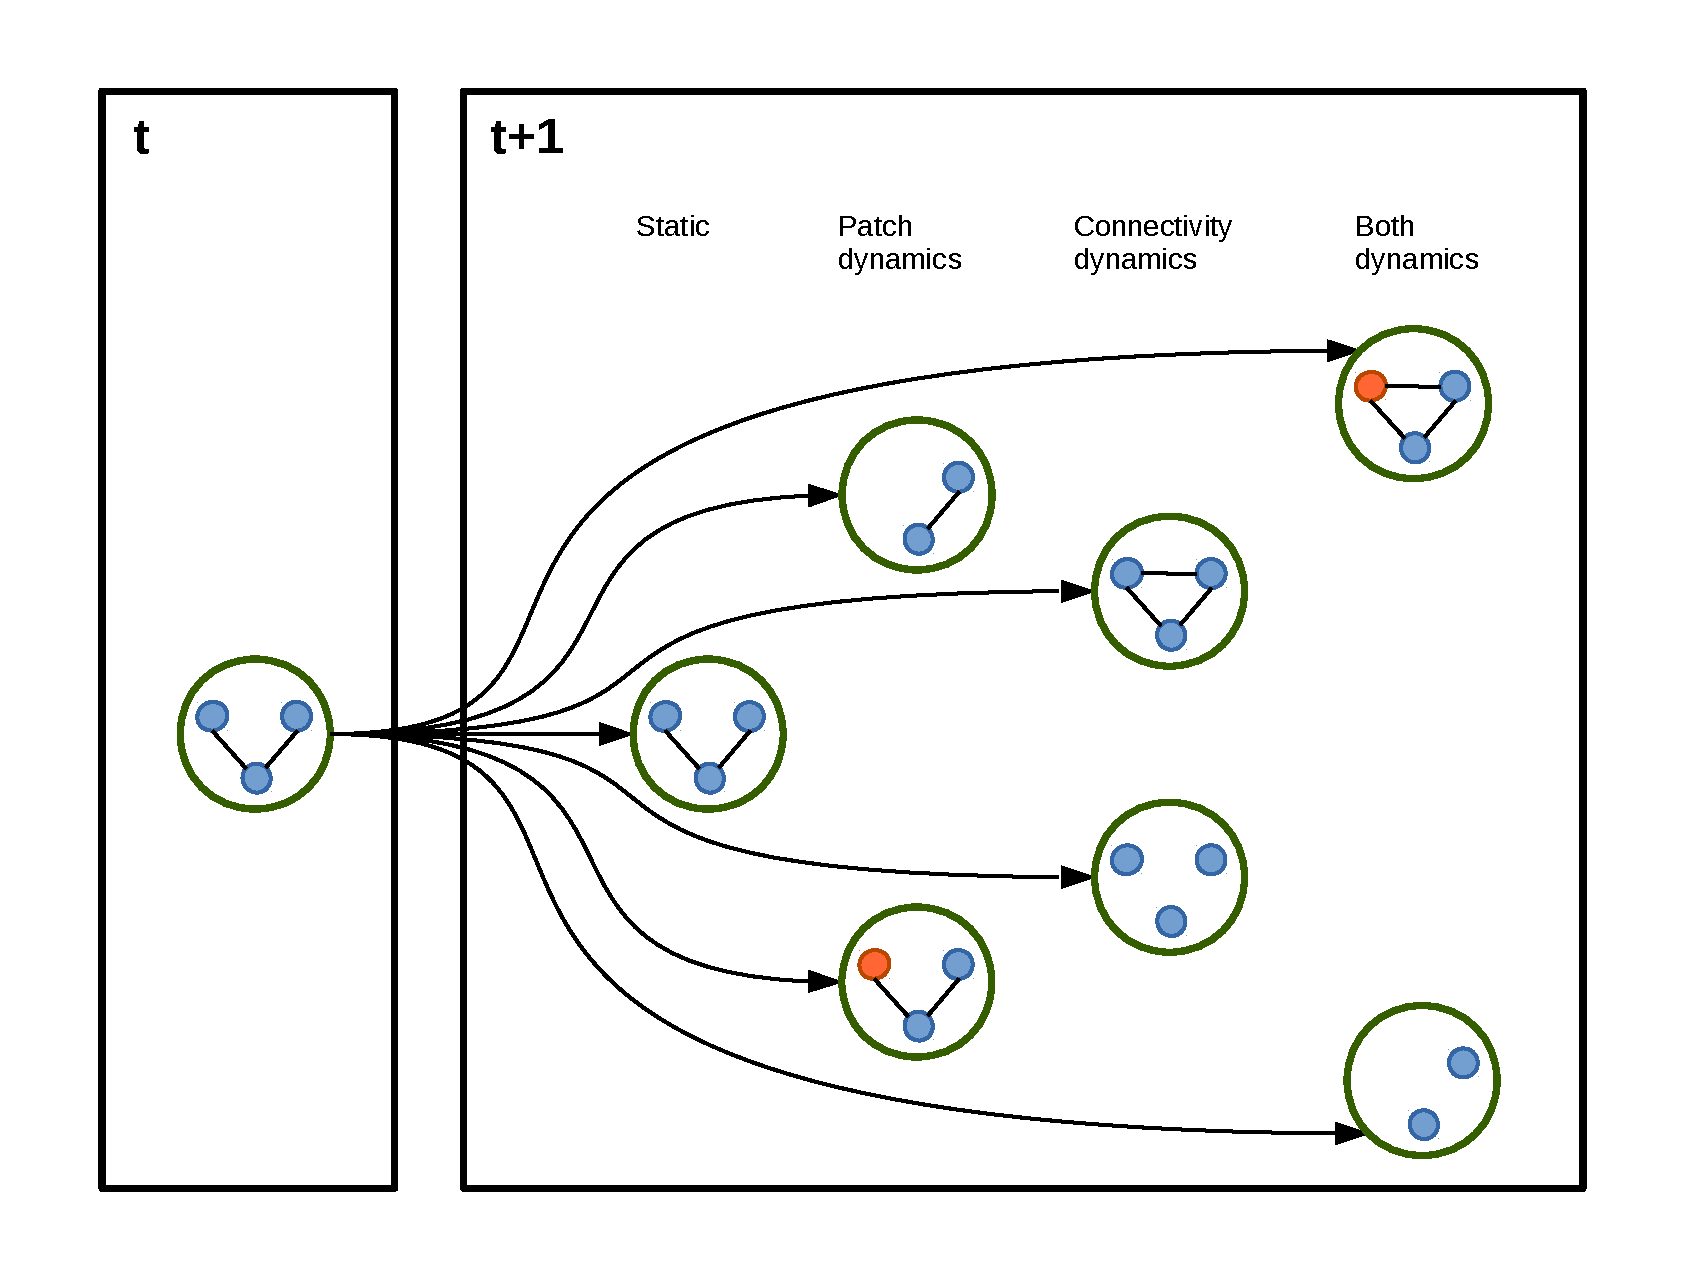
\includegraphics[height=4in,width=5in]{./figures/Figure2.eps}
\caption{}
\label{fig:Figure2}
\end{figure}

\begin{figure}[hb!]
%\begin{center}
\includegraphics[width=4in, angle=-90]{./figures/BasisForEquation.eps}
%\end{center}
\caption{}
\label{fig:Figure3}
\end{figure}

\begin{figure}[hb!]
\begin{center}
%\hspace{-0.5 in}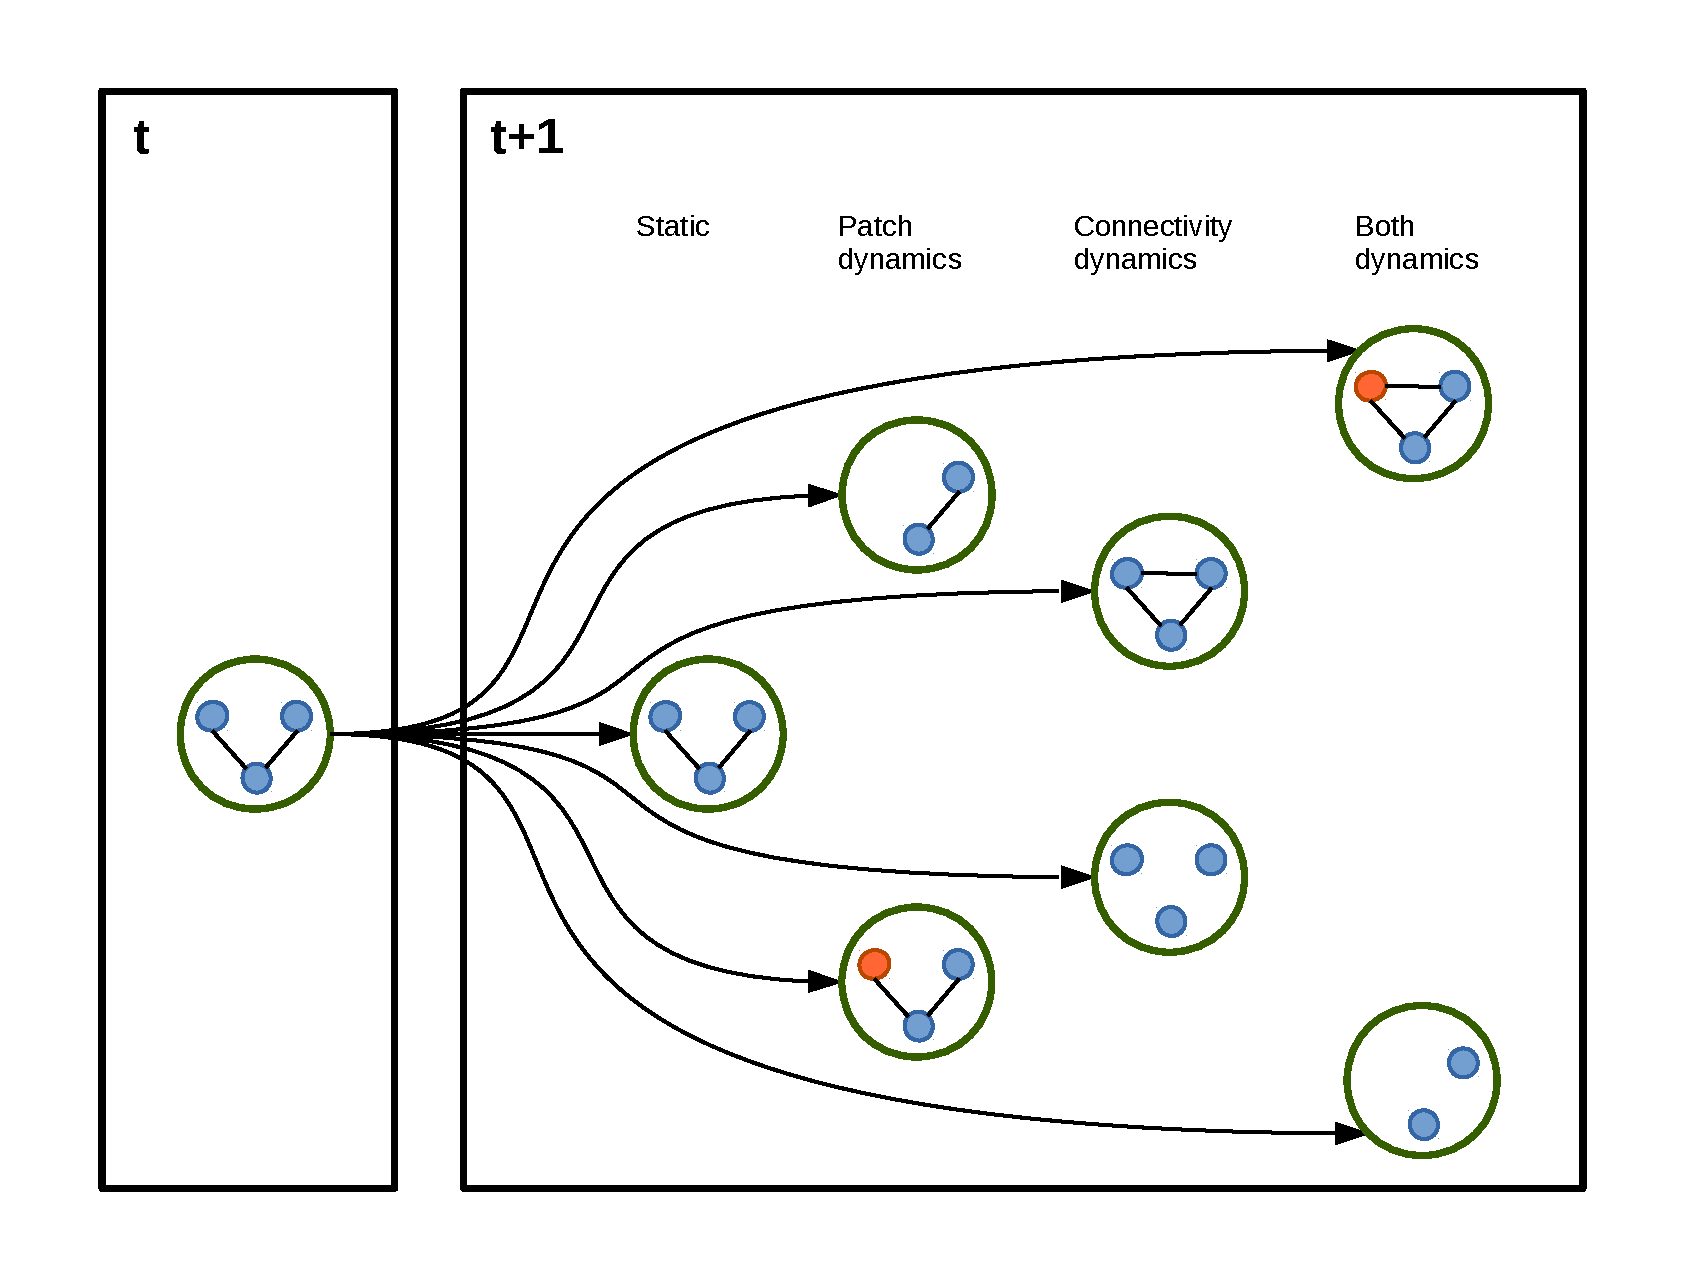
\includegraphics[width=6.75in]{./figures/Figure2.eps}
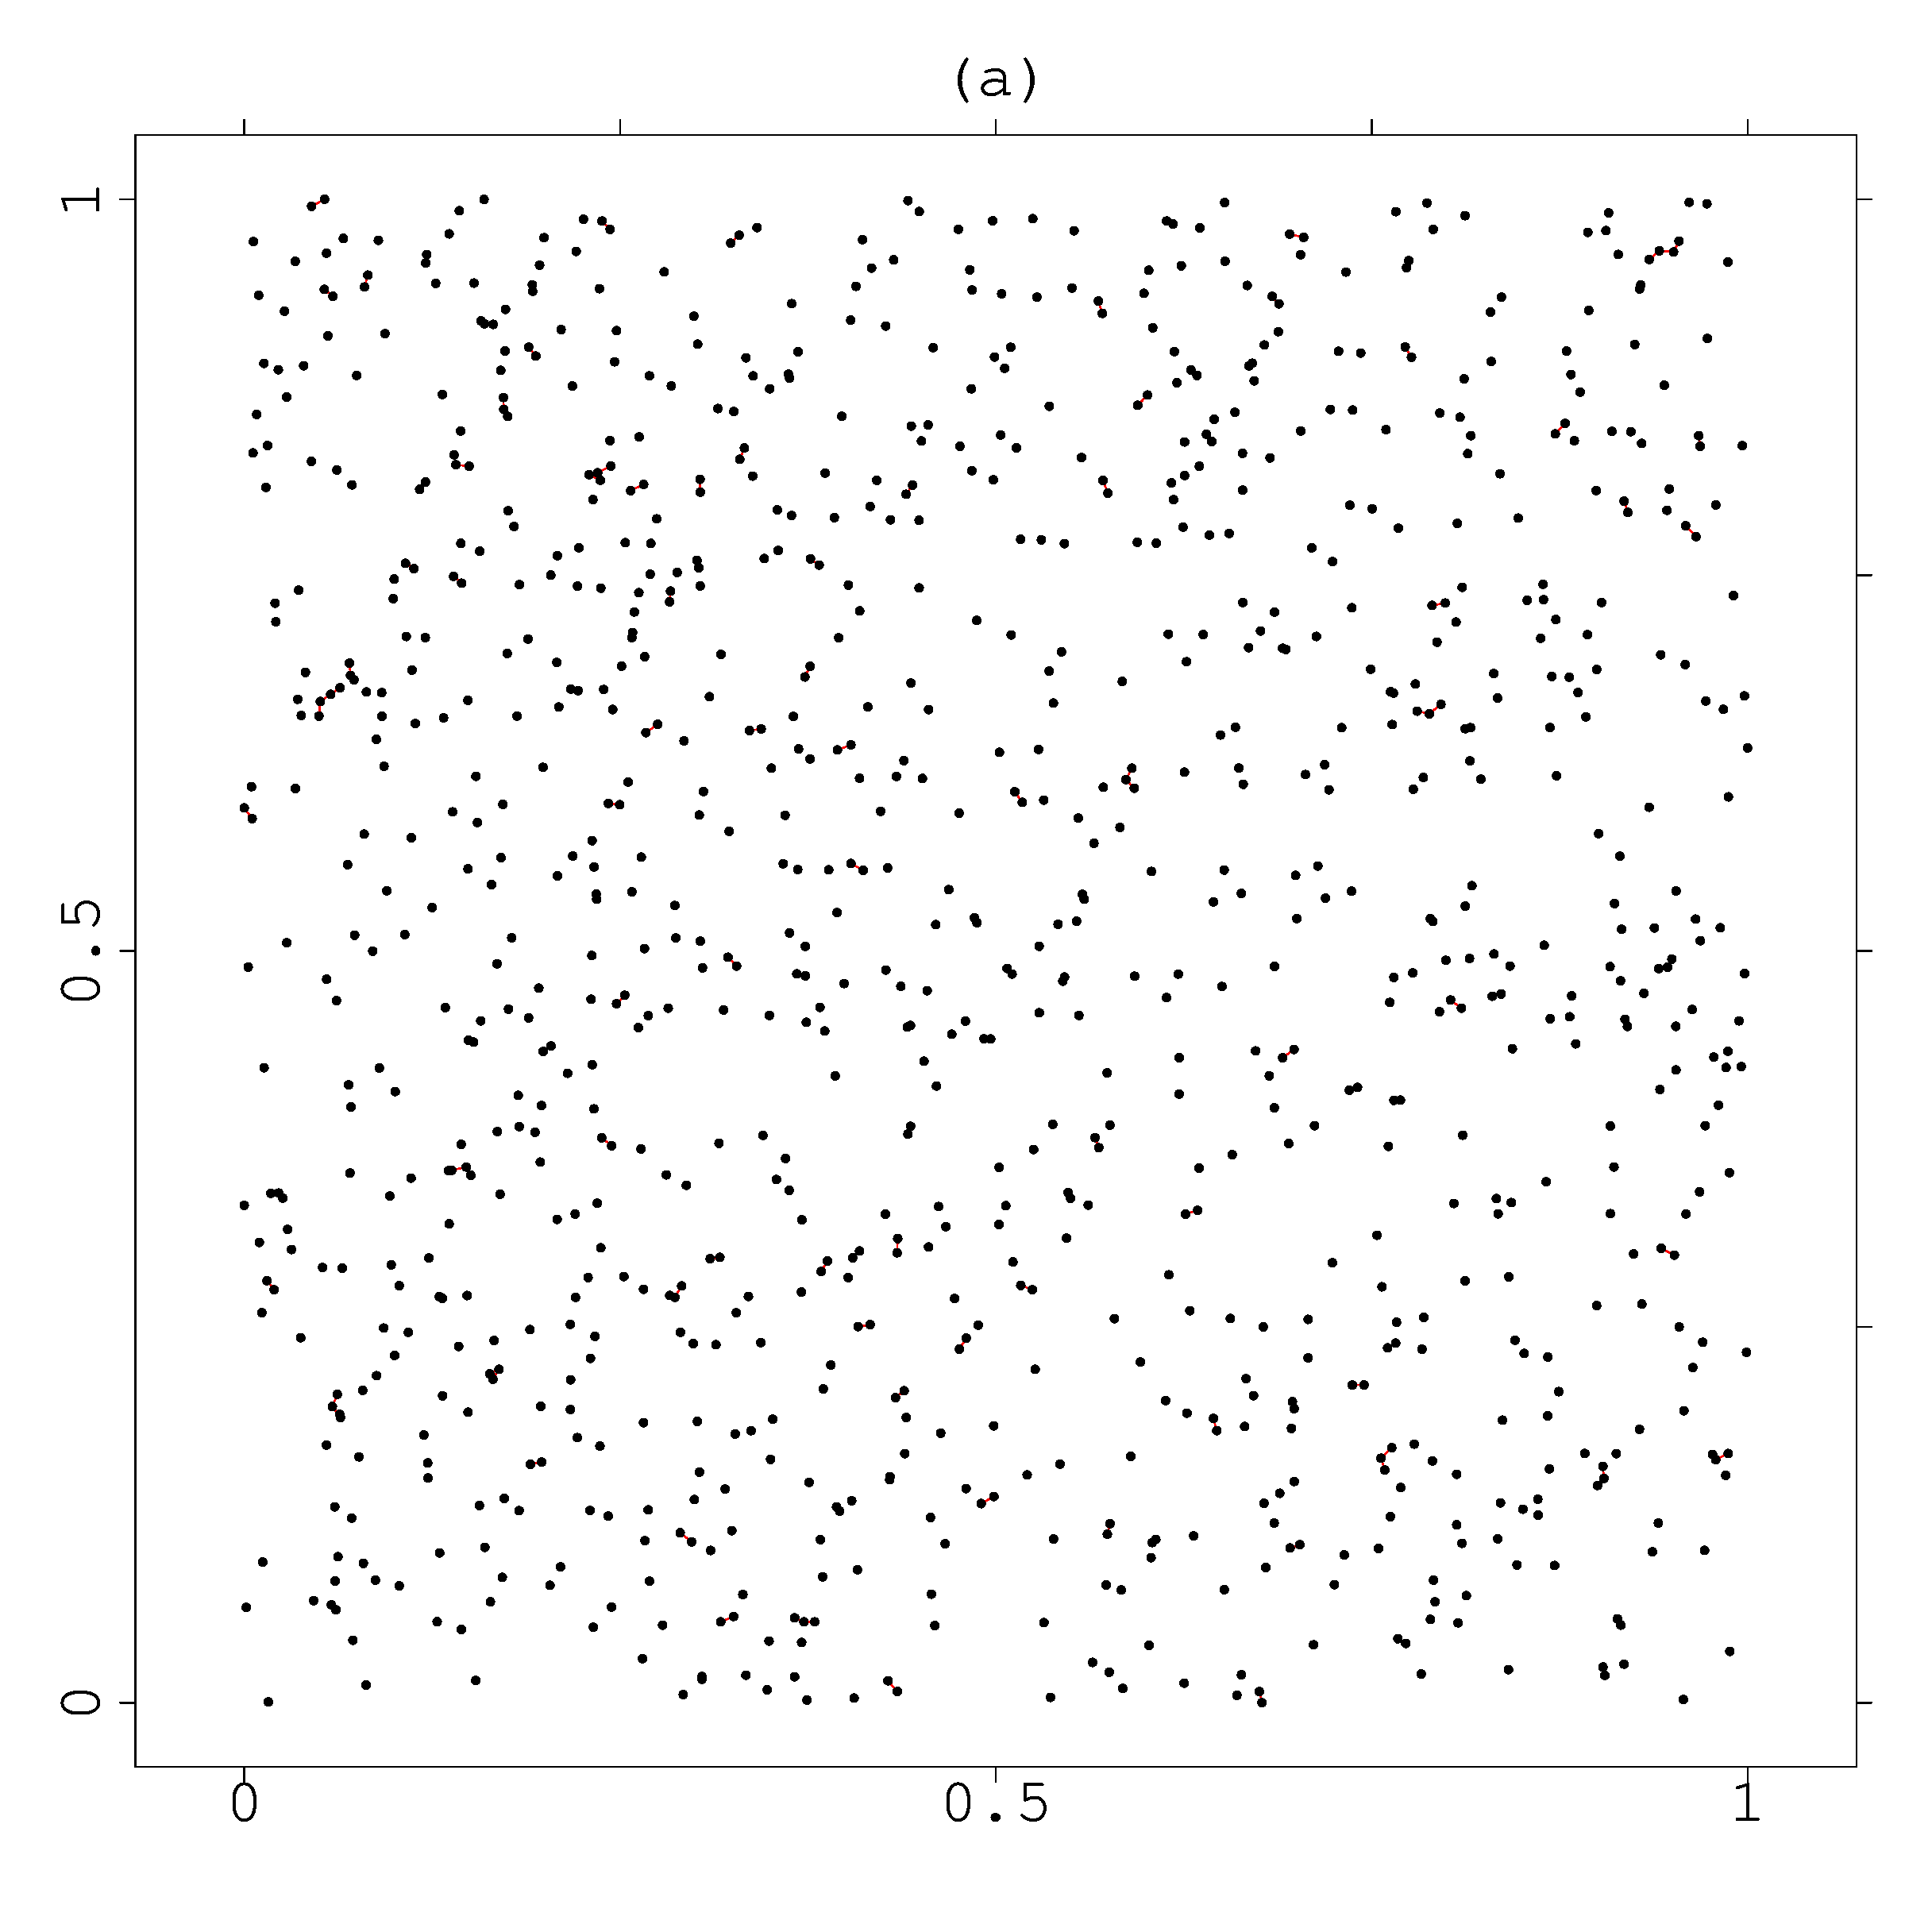
\includegraphics[width=3.1in]{./figures/RGN_r_001.eps}
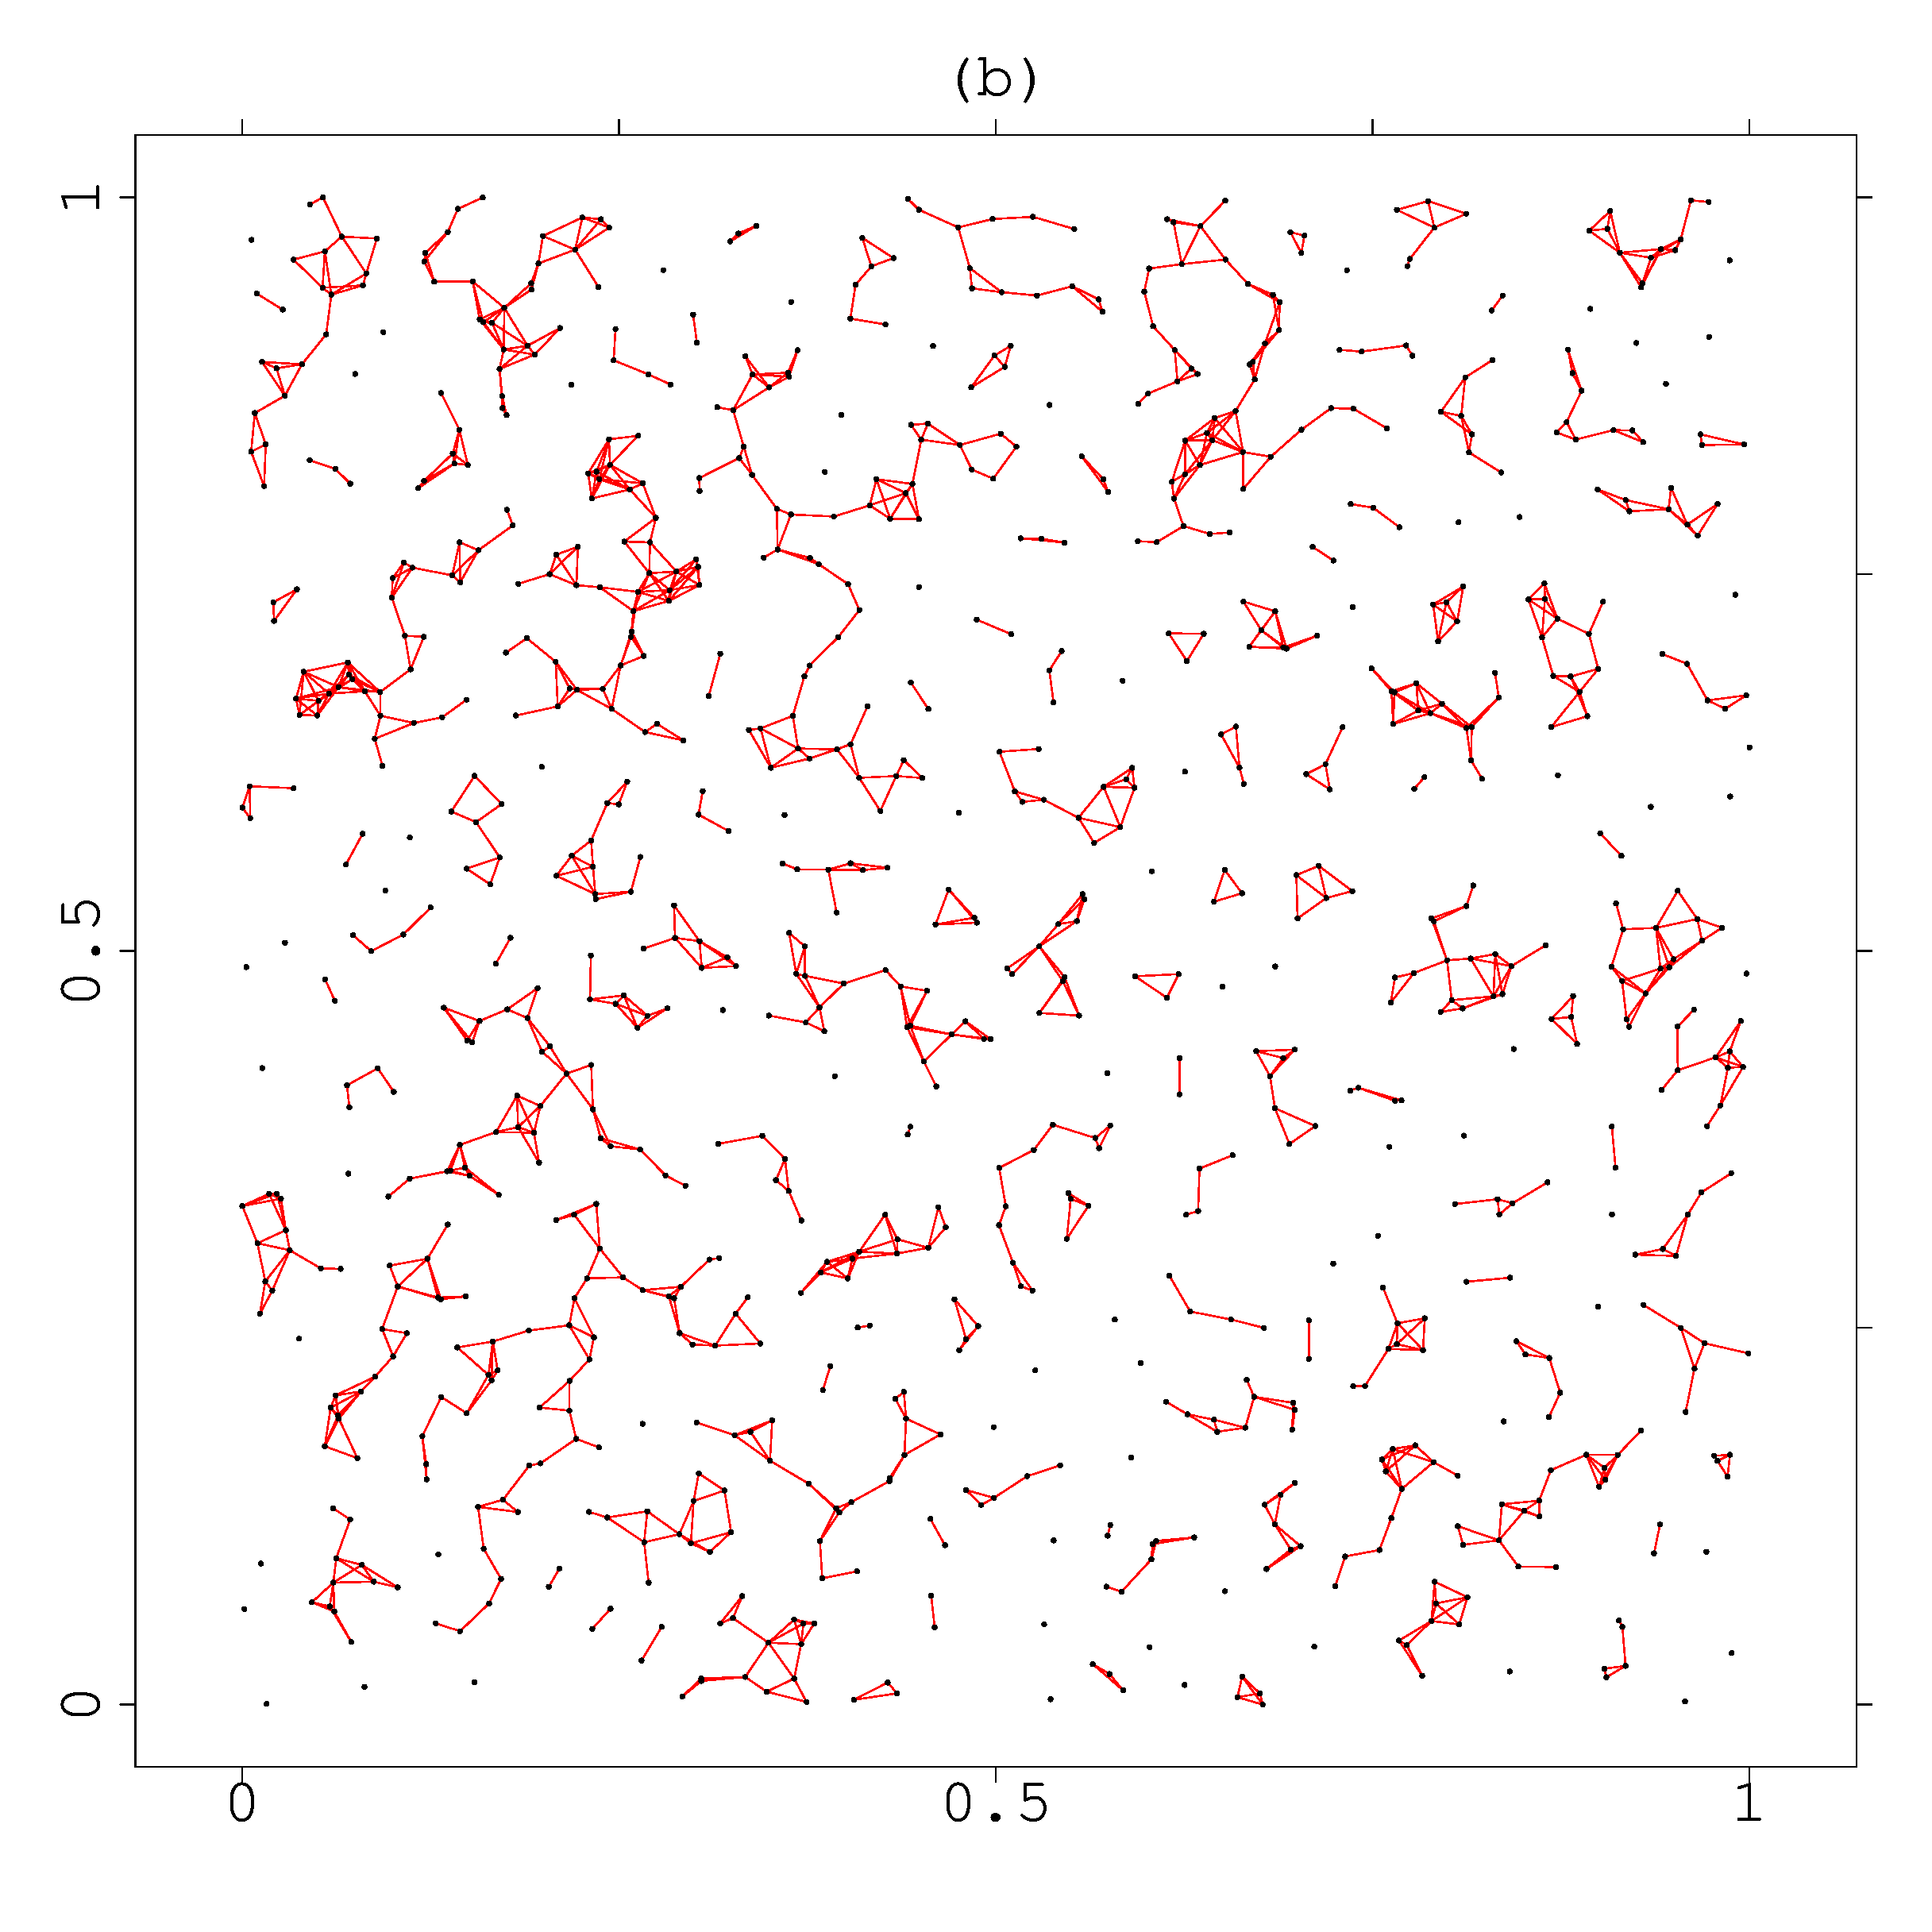
\includegraphics[width=3.1in]{./figures/RGN_r_003.eps}
\includegraphics[width=3.1in]{./figures/RGN_r_0075.eps}
\end{center}
\caption{}
\label{fig:Figure4}
\end{figure}

\begin{figure}[hb!]
\hspace{-0.5 in}\includegraphics[width=5in,angle=-90]{./figures/components_vs_gamma_5_4.eps}
\caption{}
\label{fig:Figure5}
\end{figure}

\begin{figure}[hb!]
\hspace{-0.5 in}\includegraphics[width=5in,angle=-90]{./figures/radius_vs_gamma_5_4.eps}
\caption{}
\label{fig:Figure6}
\end{figure}

\begin{figure}[hb!]
\begin{center}
\hspace{-0.5 in}\includegraphics[width=3.5in]{./figures/Figure5.eps}
\end{center}
\caption{}
\label{fig:Figure7}
\end{figure}


\appendix
% Remove brackets from numbering in List of References
\makeatletter
\renewcommand{\@biblabel}[1]{\quad#1.}
\renewcommand{\thefigure}{S\@arabic\c@figure} 
\makeatother
% Leave date blank
%\date{}
\pagestyle{myheadings}
%% ** EDIT HERE **
%% END MACROS SECTION
%\begin{document}
%\newpage

\clearpage
\begin{flushleft} 
{\Large \textbf{Appendix A from C. N. de Santana, J. Klecka, G. M. Palamara, and C. J. Meli\'{a}n, Metacommunities in dynamic landscapes}}
\end{flushleft}
\renewcommand{\theequation}{A-\arabic{equation}}
\setcounter{equation}{0}
\renewcommand{\thesection}{A\arabic{section}}
\renewcommand{\thefigure}{A\arabic{figure}}
\renewcommand{\thetable}{A\arabic{table}}
\setcounter{figure}{0}
\setcounter{table}{0}

\section*{Landscape dynamics animations}
%\vspace{2 in}
SI-A1; Sea Arctic ice cover animation (ArcticSI-A1.flv)\\
{\bf This animation shows sea Arctic ice cover from XX to XX with a time and space resolution of XX and XX, respectively. Data downloaded from XX.}
\\
\\
SI-A2; Sea Antarctic ice cover animation (AntarcticSI-A2.flv)\\
{\bf This animation shows sea Antarctic ice cover from XX to XX with a time and space resolution of XX and XX, respectively. Data downloaded from XX}
\\
SI-A3; Dynamic landscape animation (RGNSI-A3.ogv)\\
{\bf This animation shows fluctuations in landscape connectivity using amplitude, $\mathcal{A}$, and frequency, $\mathfrak{f}$ values of 1 and 0.1 (top) and 1 and 0.9 (bottom), respectively.}

\begin{comment}
\clearpage
\begin{flushleft} 
{\Large \textbf{Appendix B from C. N. de Santana, J. Klecka, G. M. Palamara, and C. J. Meli\'{a}n, Metacommunities in dynamic landscapes}}
\end{flushleft}
\renewcommand{\theequation}{B-\arabic{equation}}
\setcounter{equation}{0}
\renewcommand{\thesection}{B\arabic{section}}
\renewcommand{\thefigure}{B\arabic{figure}}
\renewcommand{\thetable}{B\arabic{table}}
\setcounter{figure}{0}
\setcounter{table}{0}

\section*{Metacommunity studies with patch and connectivity dynamics}
\vspace{2 in}
\begin{figure}
\fbox{\parbox[c]{15cm}{
\begin{tabular}{ p{1.5cm} |  p{1.5cm}  |  p{3.5cm}  | p{3.5cm} |  p{3.5cm} | p{3.5cm} }
  \hline
 & & {\textbf{Connectivity}} & & \\ \hline
  \hline                                        
 &   & \textbf{Static}  & \textbf{Random} & \textbf{Seasonal}   \\
  \hline                                        
 & {\textbf{Static}}   & Most studies  & ?  & This paper \\
 &                     &              &     & \cite{GrenfellEtAl1995_seasonality}  \\
&                                    &     &        & \cite{Ross2010}      \\
  \hline                                        
 {\textbf{Habitat}}  & {\textbf{Random}}   & \cite{Hanski1999}   & ?      & ?          \\
 &    & \cite{VuilleumierEtAl2007} &        &            \\
 &    & \cite{DrechslerJohst2010}  &        &            \\
  \hline                                        
& {\textbf{Seasonal}} & \cite{HoltCovlin1997}      & ?      & ?          \\
&                                    & \cite{LoreauEtAl2003}      &        &            \\
  \hline                                        
\end{tabular}
\caption{{\small {\bf Examples of metacommunity or
    metapopulation studies with patch and connectivity
    combinations. Studies included in the category with periodic
    connectivity changes are mostly studies of infectious diseases
    (host-parasite interactions) with seasonal variation in
    transmission rate; see also \cite{FerrariEtAl2008,
      BalcanEtAl2009_seasonal} for examples of applications for
    predicting the spread of diseases. Interrogants mean we are not
    aware of any studies addressing this combination. \carlos{THIS IS PROBABLY THE FIGURE THAT REQUIRES MORE WORK: SHOULD WE MOVE FORWARD IT OR DELETE?}}}}
\label{fig:SI-B1}
}}
\end{figure}
\end{comment}


\clearpage
\begin{flushleft} 
{\Large \textbf{Appendix B from C. N. de Santana, J. Klecka, G. M. Palamara, and C. J. Meli\'{a}n, Metacommunities in dynamic landscapes}}
\end{flushleft}

\renewcommand{\theequation}{B-\arabic{equation}}
\setcounter{equation}{0}
\renewcommand{\thesection}{B\arabic{section}}
\renewcommand{\thefigure}{B\arabic{figure}}
\renewcommand{\thetable}{B\arabic{table}}
\setcounter{figure}{0}
\setcounter{table}{0}

\section*{Stochastic metacommunity landscape dynamics}
\label{Population dispersal model}

Here, we explain in detail how we combine dispersal with local
population dynamics. The following equations conceptualize
metacommunity dynamics. The first (second) equation gives the
transition probability that the $k^{th}$ species of
metacommunity declines (increases) in abundance by one individual in
patch $i$
\begin{equation}
\begin{array}{lcr}
\hspace{-0.25 in}P \left(N_{i}^{k} - 1 | N_{i}^{k} \right) = M^{k}_{i} \left[\sum\limits^{\mathcal{P}}_{\substack{j = 1,j \ne i \\ \mathfrak{d_{ij}} \leq \mathfrak{d_{c}}}}
 \sum\limits_{k'=1,k'\ne k}^{S_{j}} m_{ij}^{k'} \left(\frac{N_{j}^{k'}}{J_{j}}\right) + \lambda \left(\frac{J_{i} - N_{i}^{k}}{J_{i} - 1}\right) + \nu \right]\\[0.5cm]
%\label{master1}
\\
\hspace{-0.25 in}P \left(N_{i}^{k} + 1 | N_{i}^{k}\right) = (1 - M^{k}_{i}) \left[
\sum\limits^{\mathcal{P}}_{\substack{j = 1,j \ne i \\ \mathfrak{d_{ij}} \leq \mathfrak{d_{c}}}}
%\sum\limits_{j=1,j\ne i}^{\mathcal{P}}
 m_{ij}^{k} \left(\frac{N_{j}^{k}}{J_{j}}\right) + \lambda \left(\frac{N_{i}^{k}}{J_{i} - 1}\right) + \nu \right].
\end{array}
\label{master}
\end{equation}
Here $M^{k}_{i}$ describes density-dependent mortality rate of species
$k$ in patch $i$. This mortality is the natural per capita mortality
rate described in this article by $\mu
\frac{N_{i}^{k}}{J_{i}}$. $N_{i}^{k}$ and $J_{i}$ are the total number of
individuals of species $k$ in patch $i$ and the total number of individuals
in patch $i$, respectively. $\mathcal{S}_{j}$ and $\mathcal{P}$ are
the total number of species in patch $j$ and the total number of
patches, respectively. In addition to the mortality rate parameters,
there are three more metacommunity specific parameters: $\lambda$, the
local birth rate, $m$, the intensity of emigration rate, and $\nu$,
the immigration rate from the regional species pool.

The first equation in (\ref{master}) gives the transition probability
for the $k^{th}$ species to decline in abundance by one individual in
patch $i$. For this to happen, an individual must die in the $k^{th}$
species, which occurs at a rate given by $M^{k}_{i}$. The first
probability inside the brackets is that of an immigration event of
some species other than $k$ from a patch different to $i$ (see
equation 2 in the main text with $\mathfrak{d_{ij}}$ the geographical
distance between patch $i$ and $j$ satisfying $\mathfrak{d_{ij}}$
$\leq$ $\mathfrak{d_{c}}$). The second term represents the probability
of having a local birth in a species other than $k$ with the -1
subtracted in the denominator after the death in the previous step of
one individual in this patch. The third term describes the probability
of an immigration event from the regional species pool. The second
equation in (\ref{master}) describes the transition probability for
the $k^{th}$ species to increase by one individual. For this to
happen, there must be no local death in species $k$ which is given by
$1 - M^{k}_{i}$. The other terms in brackets stand for dispersal (the
first term), local birth of an individual of species $k$ (second
term), and immigration of a new species $k$ from the regional species
pool. This last event can occur only when there was no such species,
i.e., when $N_{i}^{k}$ $=$ 0 at time $t - 1$.  

\clearpage
\begin{flushleft} 
{\Large \textbf{Appendix C from C. N. de Santana, J. Klecka, G. M. Palamara, and C. J. Meli\'{a}n, Metacommunities in dynamic landscapes}}
\section*{Mean $\gamma-$species richness and landscape metrics}
\end{flushleft}
\renewcommand{\theequation}{C-\arabic{equation}}
\setcounter{equation}{0}
\renewcommand{\thesection}{C\arabic{section}}
\renewcommand{\thefigure}{C\arabic{figure}}
\renewcommand{\thetable}{C\arabic{table}}
\setcounter{figure}{0}
\setcounter{table}{0}

\begin{figure}[hb!]
\begin{center}

\includegraphics[width=2.2in, angle=-90]{./figures/Figure6_Mean_a_003.eps}\hspace{-0.025 in}
\includegraphics[width=2.2in, angle=-90]{./figures/Figure6_Mean_b_003.eps}\\
\includegraphics[width=2.2in, angle=-90]{./figures/Figure6_Mean_c_003.eps}\hspace{-0.025 in}
\includegraphics[width=2.2in, angle=-90]{./figures/Figure6_Mean_d_003.eps}\\

\end{center}
\caption{This figure shows the mean $\gamma-$species richness as a function of amplitude, $\mathcal{A}$, and frequency, $\mathfrak{f}$, for four landscape metrics. (a) Isoclines values represent the mean landscape connectivity calculated as $2\sum_{i}^{\mathcal{P}} \Gamma_{i}/(\mathcal{P}(\mathcal{P} - 1))$, with $\mathcal{P}$, the total number of patches, and $\Gamma_{i}$, the connectivity of patch $i$. (b) Isoclines values represent the mean number of components, $\hat{\mathcal{C}}$. (c) Isoclines values represent the mean landscape continuity, calculated as ($\mathcal{P} - \mathcal{C}$)/$\mathcal{P}$, with $\mathcal{P}$, the total number of patches, and $\mathcal{C}$ the number of components. (d) Isoclines values represent the mean landscape availability calculated as the ratio between landscape connectivity and landscape continuity. Simulations were done for emigration rate, $\mathrm{m}$ = 0.1, immigration rate from the species regional pool, $\mathrm{\nu}$ = 0.003, total number of patches, $\mathcal{P}$ = 100, patch size, $J_{x_i,y_i}$ = 100 individuals and number of generations per replicate, $\mathcal{G}$ = 1000. $\gamma-$species richness was averaged over the last 500 generations in each replicate.}
\label{fig:SI-C1}
\end{figure}

\clearpage
\begin{flushleft} 
{\Large \textbf{Appendix D from C. N. de Santana, J. Klecka, G. M. Palamara, and C. J. Meli\'{a}n, Metacommunities in dynamic landscapes}}
\section*{Mean $\gamma-$species richness}
\end{flushleft}
\renewcommand{\theequation}{D-\arabic{equation}}
\setcounter{equation}{0}
\renewcommand{\thesection}{D\arabic{section}}
\renewcommand{\thefigure}{D\arabic{figure}}
\renewcommand{\thetable}{D\arabic{table}}
\setcounter{figure}{0}
\setcounter{table}{0}

\begin{figure}[hb!]
\begin{center}
%\begin{tabular}{cc}
\includegraphics[width=2.5in]{./figures/new_A_r0_MeanGamma_001.eps}\hspace{-0.025 in}
\includegraphics[width=2.5in]{./figures/new_A_r0_MeanGamma_004.eps}\\
\includegraphics[width=2.5in]{./figures/new_A_r0_MeanGamma_007.eps}\hspace{-0.025 in}
\includegraphics[width=2.5in]{./figures/new_A_r0_MeanGamma_010.eps}\\
%\end{tabular}
\end{center}
\caption{This figure shows the mean $\gamma-$species richness as a function of the dispersal radius, $\mathfrak{d_{c}}$), and amplitude, $\mathcal{A}$, for static (black, $\mathcal{A}$ = 0), coupled dynamic (blue, $\mathcal{A}$ = $\mathfrak{d_{0}}$), and dynamic landscapes (red, $\mathcal{A}$ = 1) for four frequency, $\mathfrak{f}$, values, (a) $0.001$, (b) $0.01$, (c) $0.1$ , and (d) $1$. Vertical dotted line represents the critical threshold in static landscapes. Isoclines (dotted lines) represent the mean number of components, $\hat{\mathcal{C}}$, for each combination of dispersal radius, $\mathfrak{d_{c}}$, and amplitude $\mathcal{A}$. Simulations were done for emigration rate, $\mathrm{m}$ = 0.1, immigration rate from the species regional pool, $\mathrm{\nu}$ = 0.003, total number of patches, $\mathcal{P}$ = 100, patch size, $J_{x_i,y_i}$ = 100 individuals and number of generations per replicate, $\mathcal{G}$ = 1000. Values plotted represent the mean values over the last 500 generations in each replicate.}
\label{fig:SI-D1}
\end{figure}

\begin{figure}[hb!]
\hspace{-0.5 in}\includegraphics[width=5in,angle=-90]{./figures/components_vs_gamma_3_2.eps}
\caption{}
\label{fig:SI-D2}
\end{figure}

\begin{figure}[hb!]
\hspace{-0.5 in}\includegraphics[width=5in,angle=-90]{./figures/radius_vs_gamma_3_2.eps}
\caption{}
\label{fig:SI-D3}
\end{figure}

\end{document}